%\documentclass{standalone}\usepackage{tikz}\begin{document}


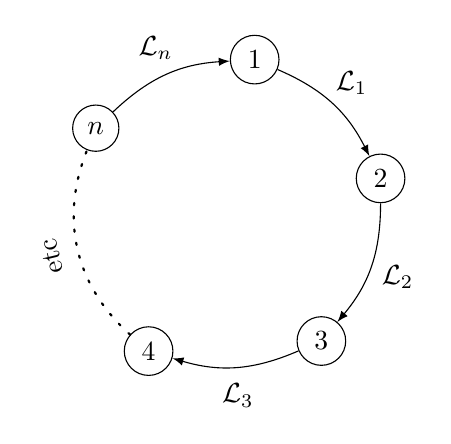
\begin{tikzpicture}

\def \margin{4mm}
\def \radius {2cm}
\def \labelsep {3mm}
\def \dotsep {.4mm}
\def \bend {20}
\def \dotbend {35}
\def \dotmargin {15}

\def \n {4}

\foreach \i in {1,...,\n}
{
  \node (\i) [draw,circle] at ({180 - 360/(\n + 1.4) * (\i +.5)}:\radius) {\i};
}

\foreach \i [remember=\i as \lasti (initially 1)] in {2,...,\n}
{
  \draw[->, >=latex] (\lasti) to[bend left=\bend] (\i);
  \node at ({180 - 360/(\n + 1.4) * (\i +.5 - .5)}:{\radius + \labelsep}) {$\mathcal{L}_\lasti$};
  \node at ({0 + (360/(\n + 1.4) * (\i +.5 - .5))}:{\radius + \labelsep}) {\hphantom{$\mathcal{L}_\lasti$}};
}

\node (n) [draw, circle] at ({180 - 360/(\n + 1.4) * (0 +.5)}:\radius) {$n$};

\draw[->, >=latex] (n) to[bend left=\bend] (1);
\node at ({180 - 360/(\n + 1.4) * (1 +.5 - .5)}:{\radius + \labelsep}) {$\mathcal{L}_n$};

\node[rotate=(( - 360/(\n + 1.4) * (\n/2 + .5)) - 90)] at ({(-360/(\n + 1.4) * (\n/2 + .5))}:{\radius + \labelsep}) {etc};

\draw[thick,line cap=round,loosely dotted, >=latex] (\n) to[bend left=\dotbend] (n);
%\draw[thick,line cap=round,loosely dotted] ({360/(\n + 1.4) * (0 +.5) - \dotmargin}:{\radius - \dotsep}) arc ((360/(\n + 1.4) * (0 +.5))+360 - \dotmargin:(360/(\n + 1.4) * (4 +.5)) + \dotmargin:\radius - \dotsep);


%\draw[color=red] (0:\radius) arc (0:360:\radius);

%\node (1) [draw, circle] at (0,0) {$1$};
%\node (2) [draw, circle] at ({\width},0) {$2$};
%\draw[->, >=latex] (1) -- node[above] {$\mathcal{L}_1$} (2);

\end{tikzpicture}


%\end{document}